\documentclass[11pt]{article}

\usepackage[margin=1in]{geometry}
\usepackage{graphicx}
\usepackage{booktabs}
\usepackage{hyperref}
\usepackage{caption}
\usepackage{subcaption}
\usepackage{parskip}

\title{OfficeHours AI --- Mid-Progress Report}
\author{OfficeHours AI Project Team}
\date{June 2026}

\begin{document}

\maketitle

\begin{abstract}
OfficeHours AI is an AI-assisted office-hours triage prototype for finals-week
academic support. This mid-report documents the implemented student kiosk,
professor dashboard, backend API, classification and clustering pipeline, and
initial verification assets. Screenshots from a seeded demo session illustrate
the end-to-end workflow.
\end{abstract}

\section{Project overview}
Professors receive many repeated questions during peak exam periods, while
students may hesitate to seek help because of stress or privacy concerns.
OfficeHours AI groups similar requests, recommends response actions, and keeps
the professor in control of final decisions.

\section{Research question}
Can an AI-assisted office-hours triage system reduce faculty communication
overload and improve student comfort in seeking academic help during final exam
periods?

\section{System architecture}
The prototype consists of four major components:
\begin{itemize}
  \item \textbf{Student kiosk} --- barcode/manual check-in, anonymous or identified submission, confirmation and status lookup.
  \item \textbf{Professor dashboard} --- request queue, charts, recommendation cards, office-hours setup.
  \item \textbf{Backend API} --- FastAPI, SQLite, request CRUD, classification, clustering, action orchestration.
  \item \textbf{AI/NLP layer} --- rule-based classifier and sentence-transformer clustering (lexical backend for tests).
\end{itemize}

\section{Implementation progress}
At mid-semester the project includes backend persistence, both frontends, CI,
synthetic datasets, semantic clustering, barcode check-in, recommendation cards,
action orchestration, demo seeding, and evaluation survey templates.

\section{Demo screenshots}
Figures~\ref{fig:kiosk-checkin}--\ref{fig:ci} show the seeded finals-week demo.
Captions follow \path{demo/screenshots/README.md}.

\begin{figure}[htbp]
  \centering
  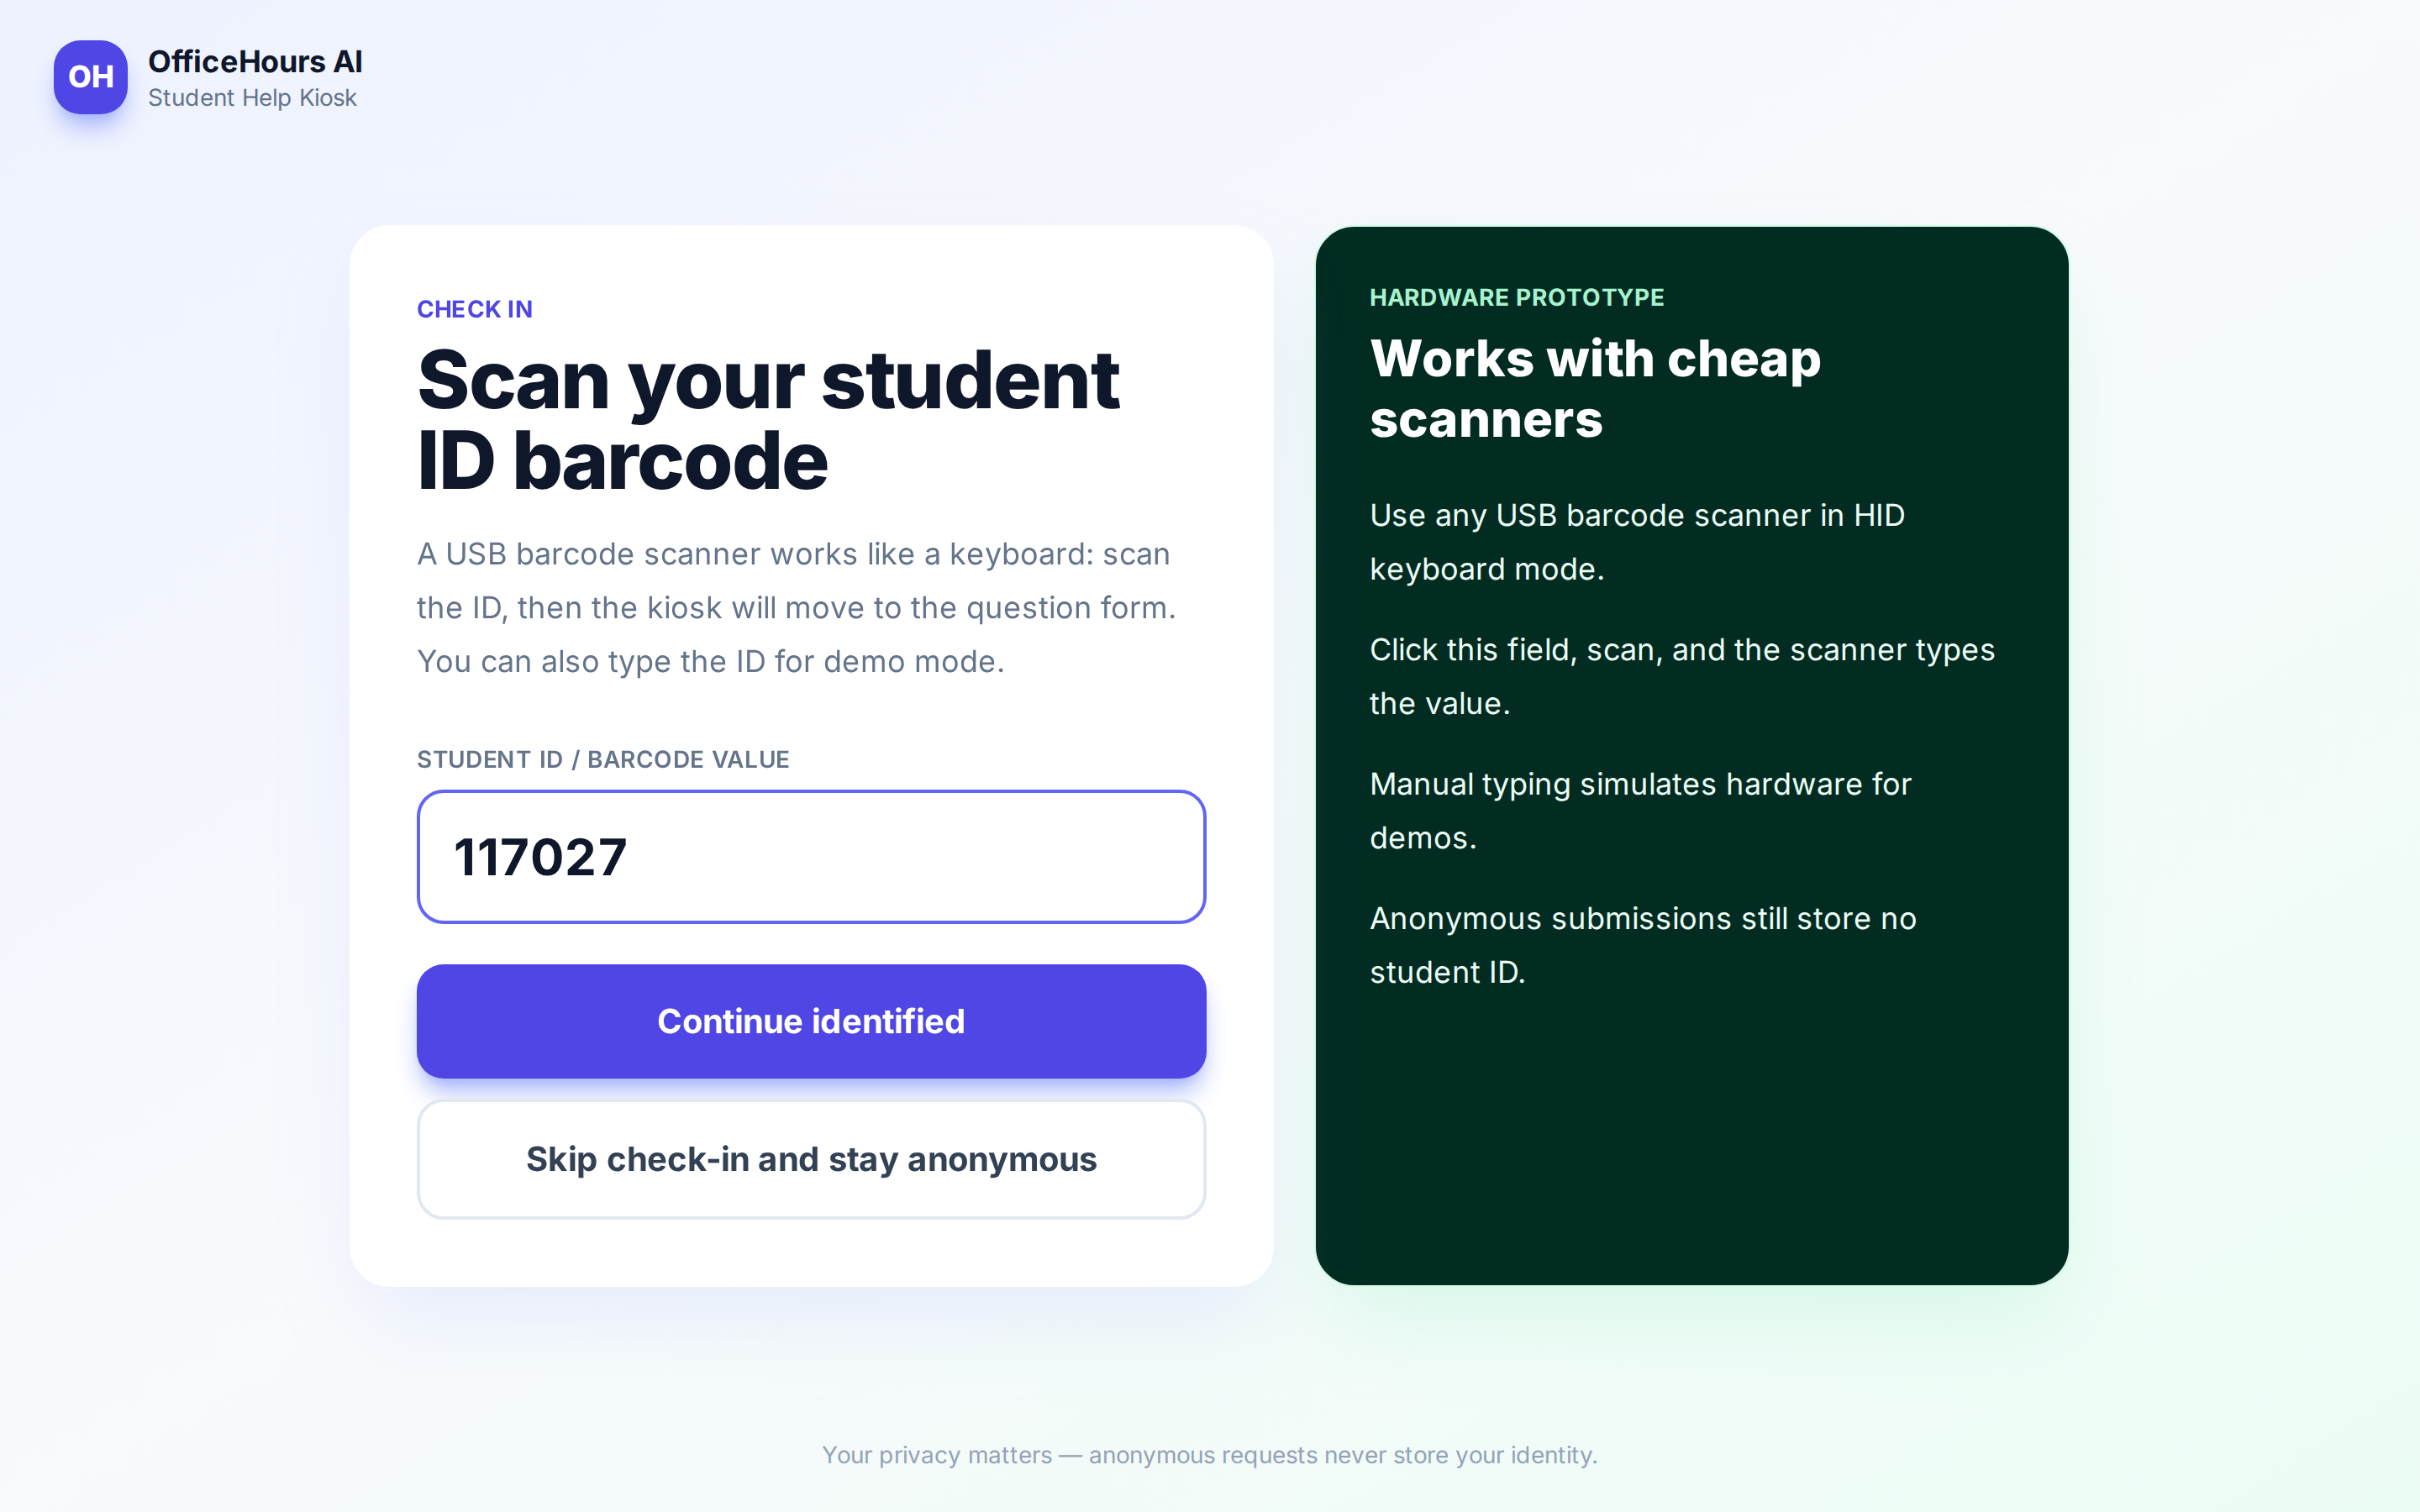
\includegraphics[width=0.92\linewidth]{../../demo/screenshots/01-student-kiosk-checkin.png}
  \caption{Scanner-compatible student check-in flow.}
  \label{fig:kiosk-checkin}
\end{figure}

\begin{figure}[htbp]
  \centering
  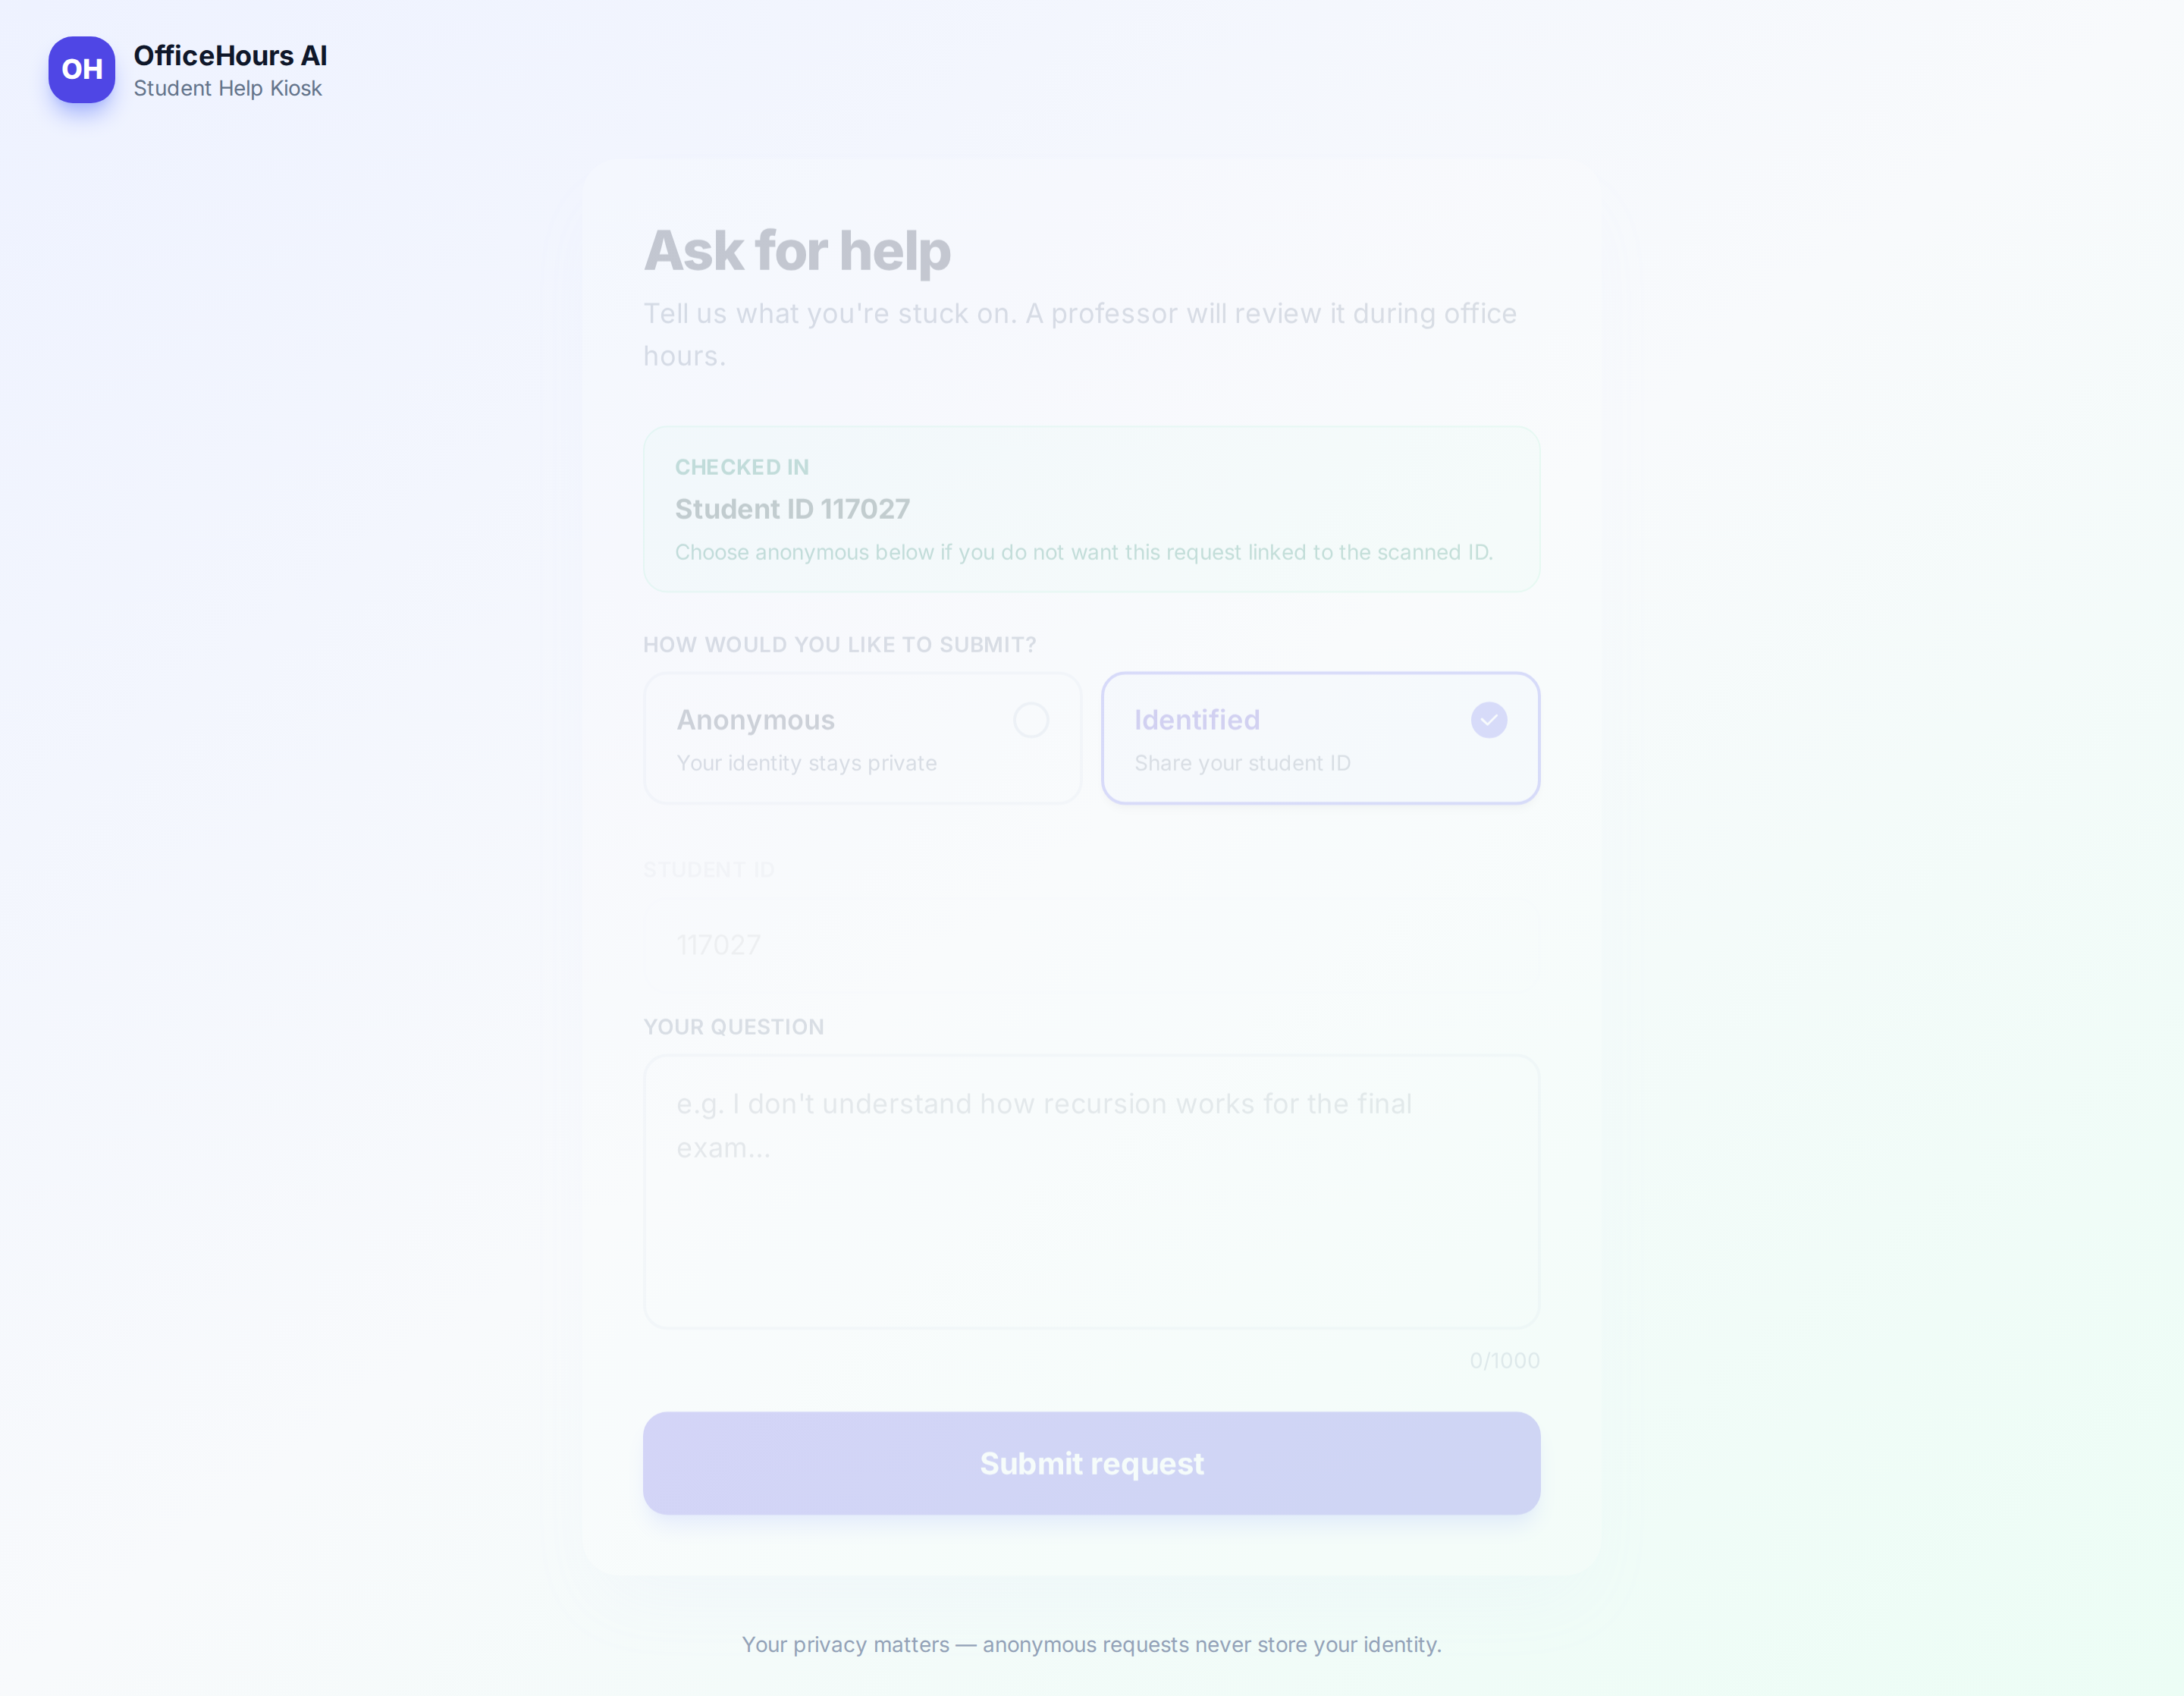
\includegraphics[width=0.92\linewidth]{../../demo/screenshots/02-student-request-form.png}
  \caption{Privacy-preserving request submission.}
  \label{fig:request-form}
\end{figure}

\begin{figure}[htbp]
  \centering
  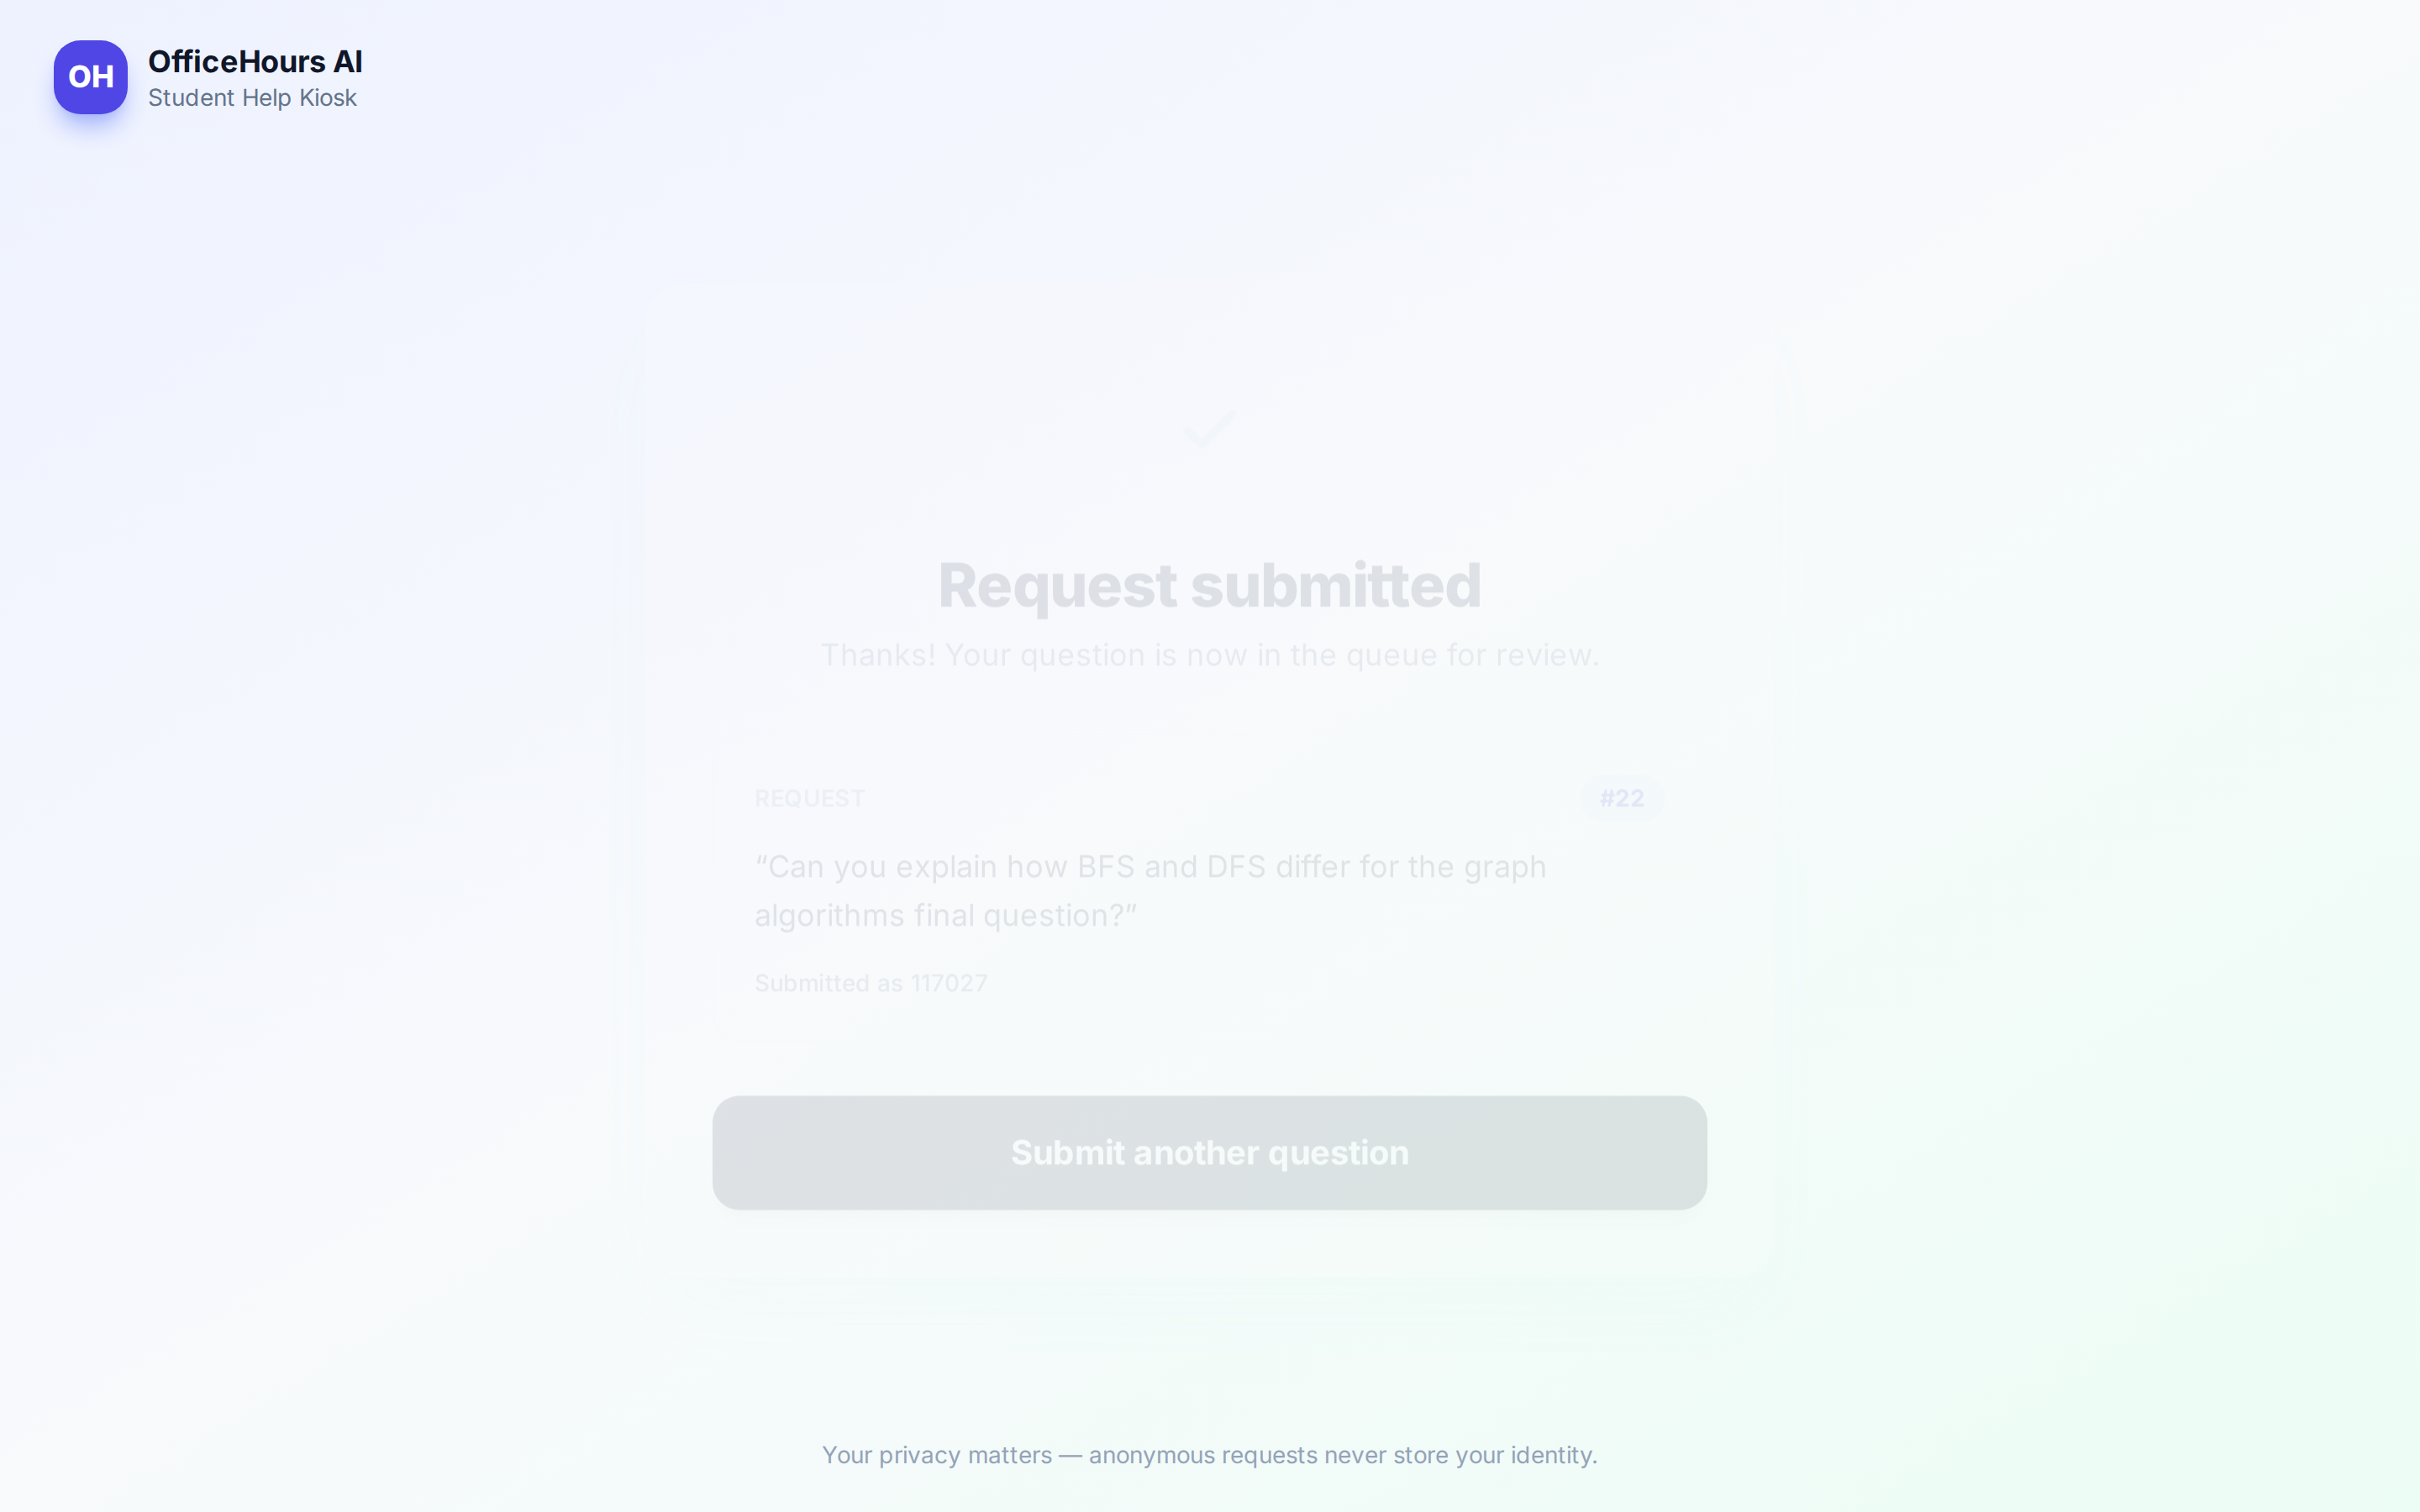
\includegraphics[width=0.92\linewidth]{../../demo/screenshots/03-submission-confirmation.png}
  \caption{Student receives confirmation after backend submission.}
  \label{fig:confirmation}
\end{figure}

\begin{figure}[htbp]
  \centering
  
\includegraphics[width=0.85\linewidth]{../../demo/screenshots/04-professor-dashboard-overview.png}
  \caption{Professor sees categorized and clustered request queue.}
  \label{fig:dashboard}
\end{figure}

\begin{figure}[htbp]
  \centering
  
\includegraphics[width=0.85\linewidth]{../../demo/screenshots/05-recommendation-cards.png}
  \caption{AI-assisted recommendations group repeated requests into actions.}
  \label{fig:recommendations}
\end{figure}

\begin{figure}[htbp]
  \centering
  
\includegraphics[width=0.85\linewidth]{../../demo/screenshots/06-action-orchestration-plan.png}
  \caption{Professor decision triggers a next-step action plan.}
  \label{fig:action-plan}
\end{figure}

\begin{figure}[htbp]
  \centering
  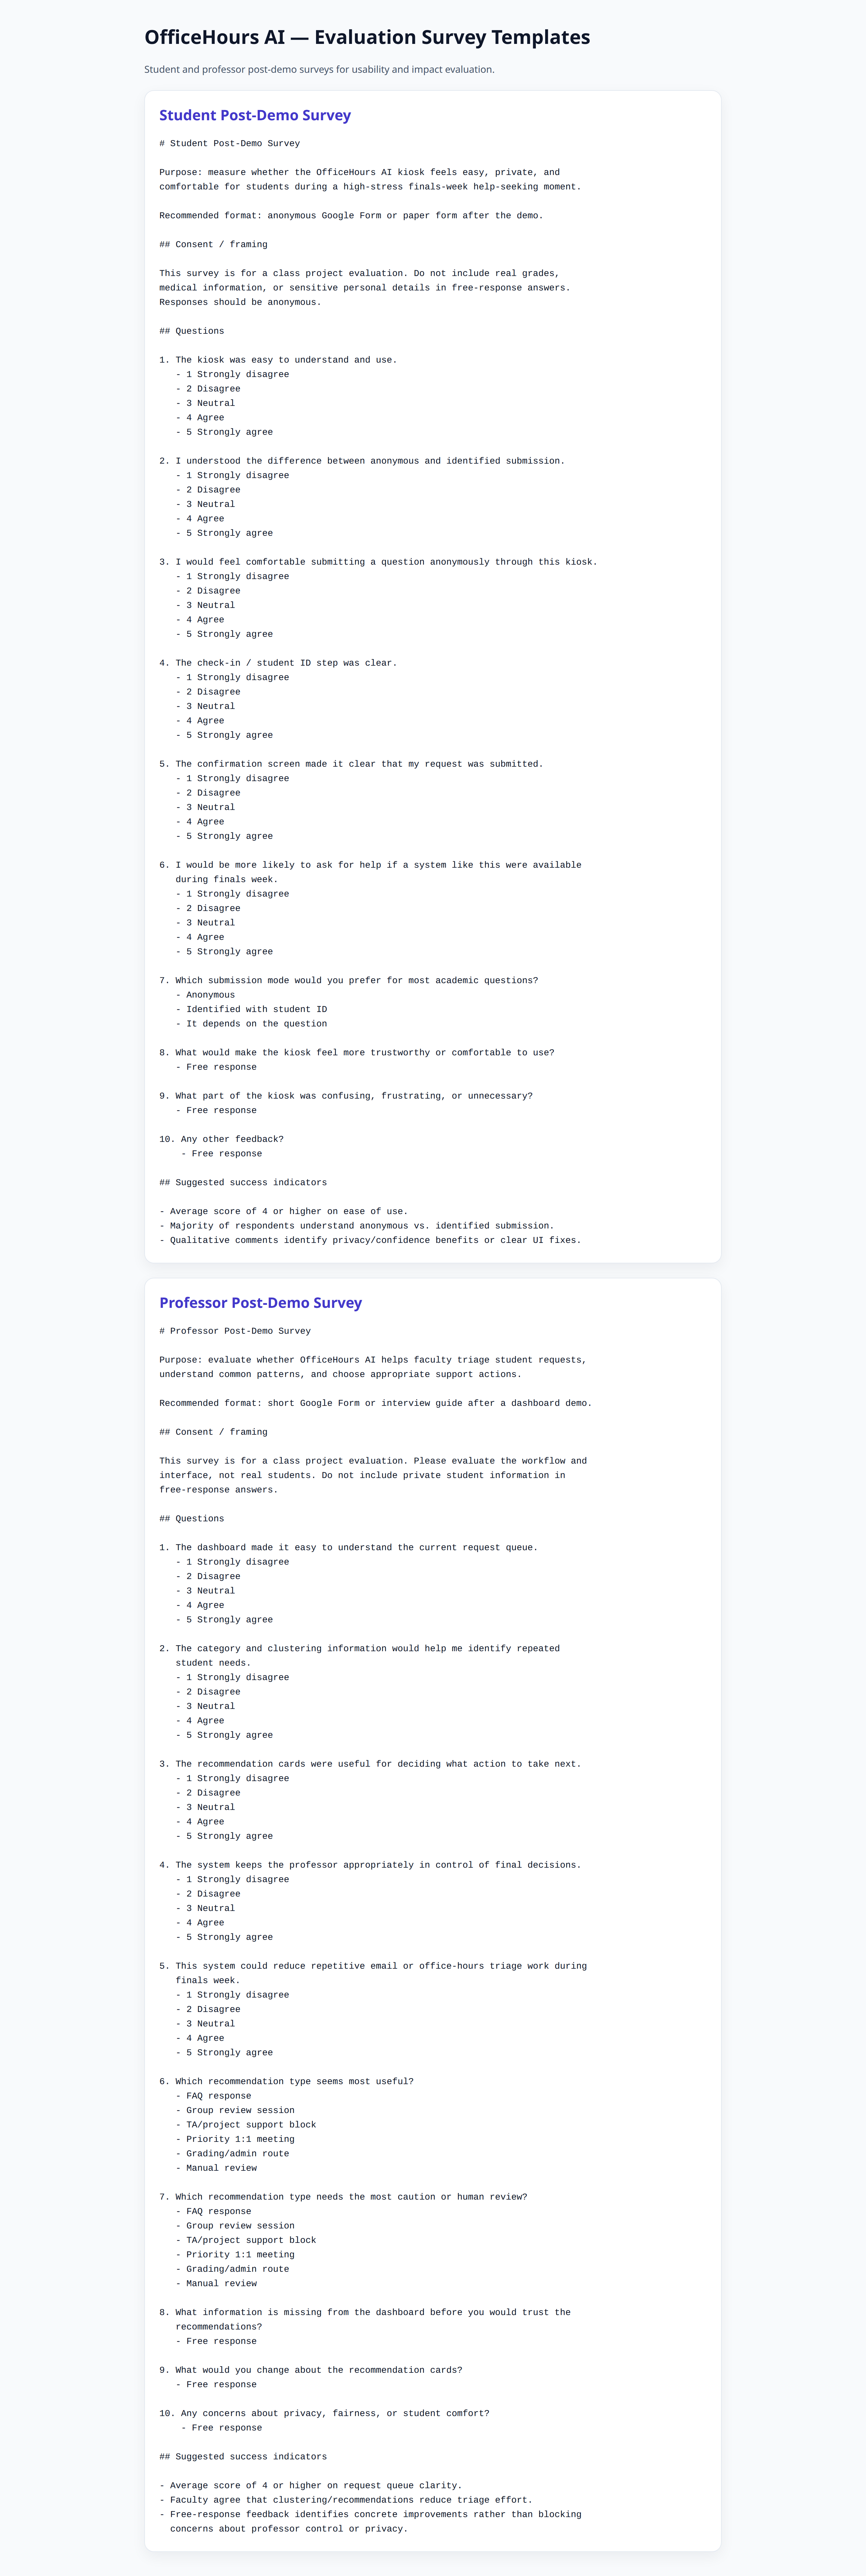
\includegraphics[width=0.92\linewidth]{../../demo/screenshots/07-survey-templates.png}
  \caption{Evaluation instruments for student and professor feedback.}
  \label{fig:surveys}
\end{figure}

\begin{figure}[htbp]
  \centering
  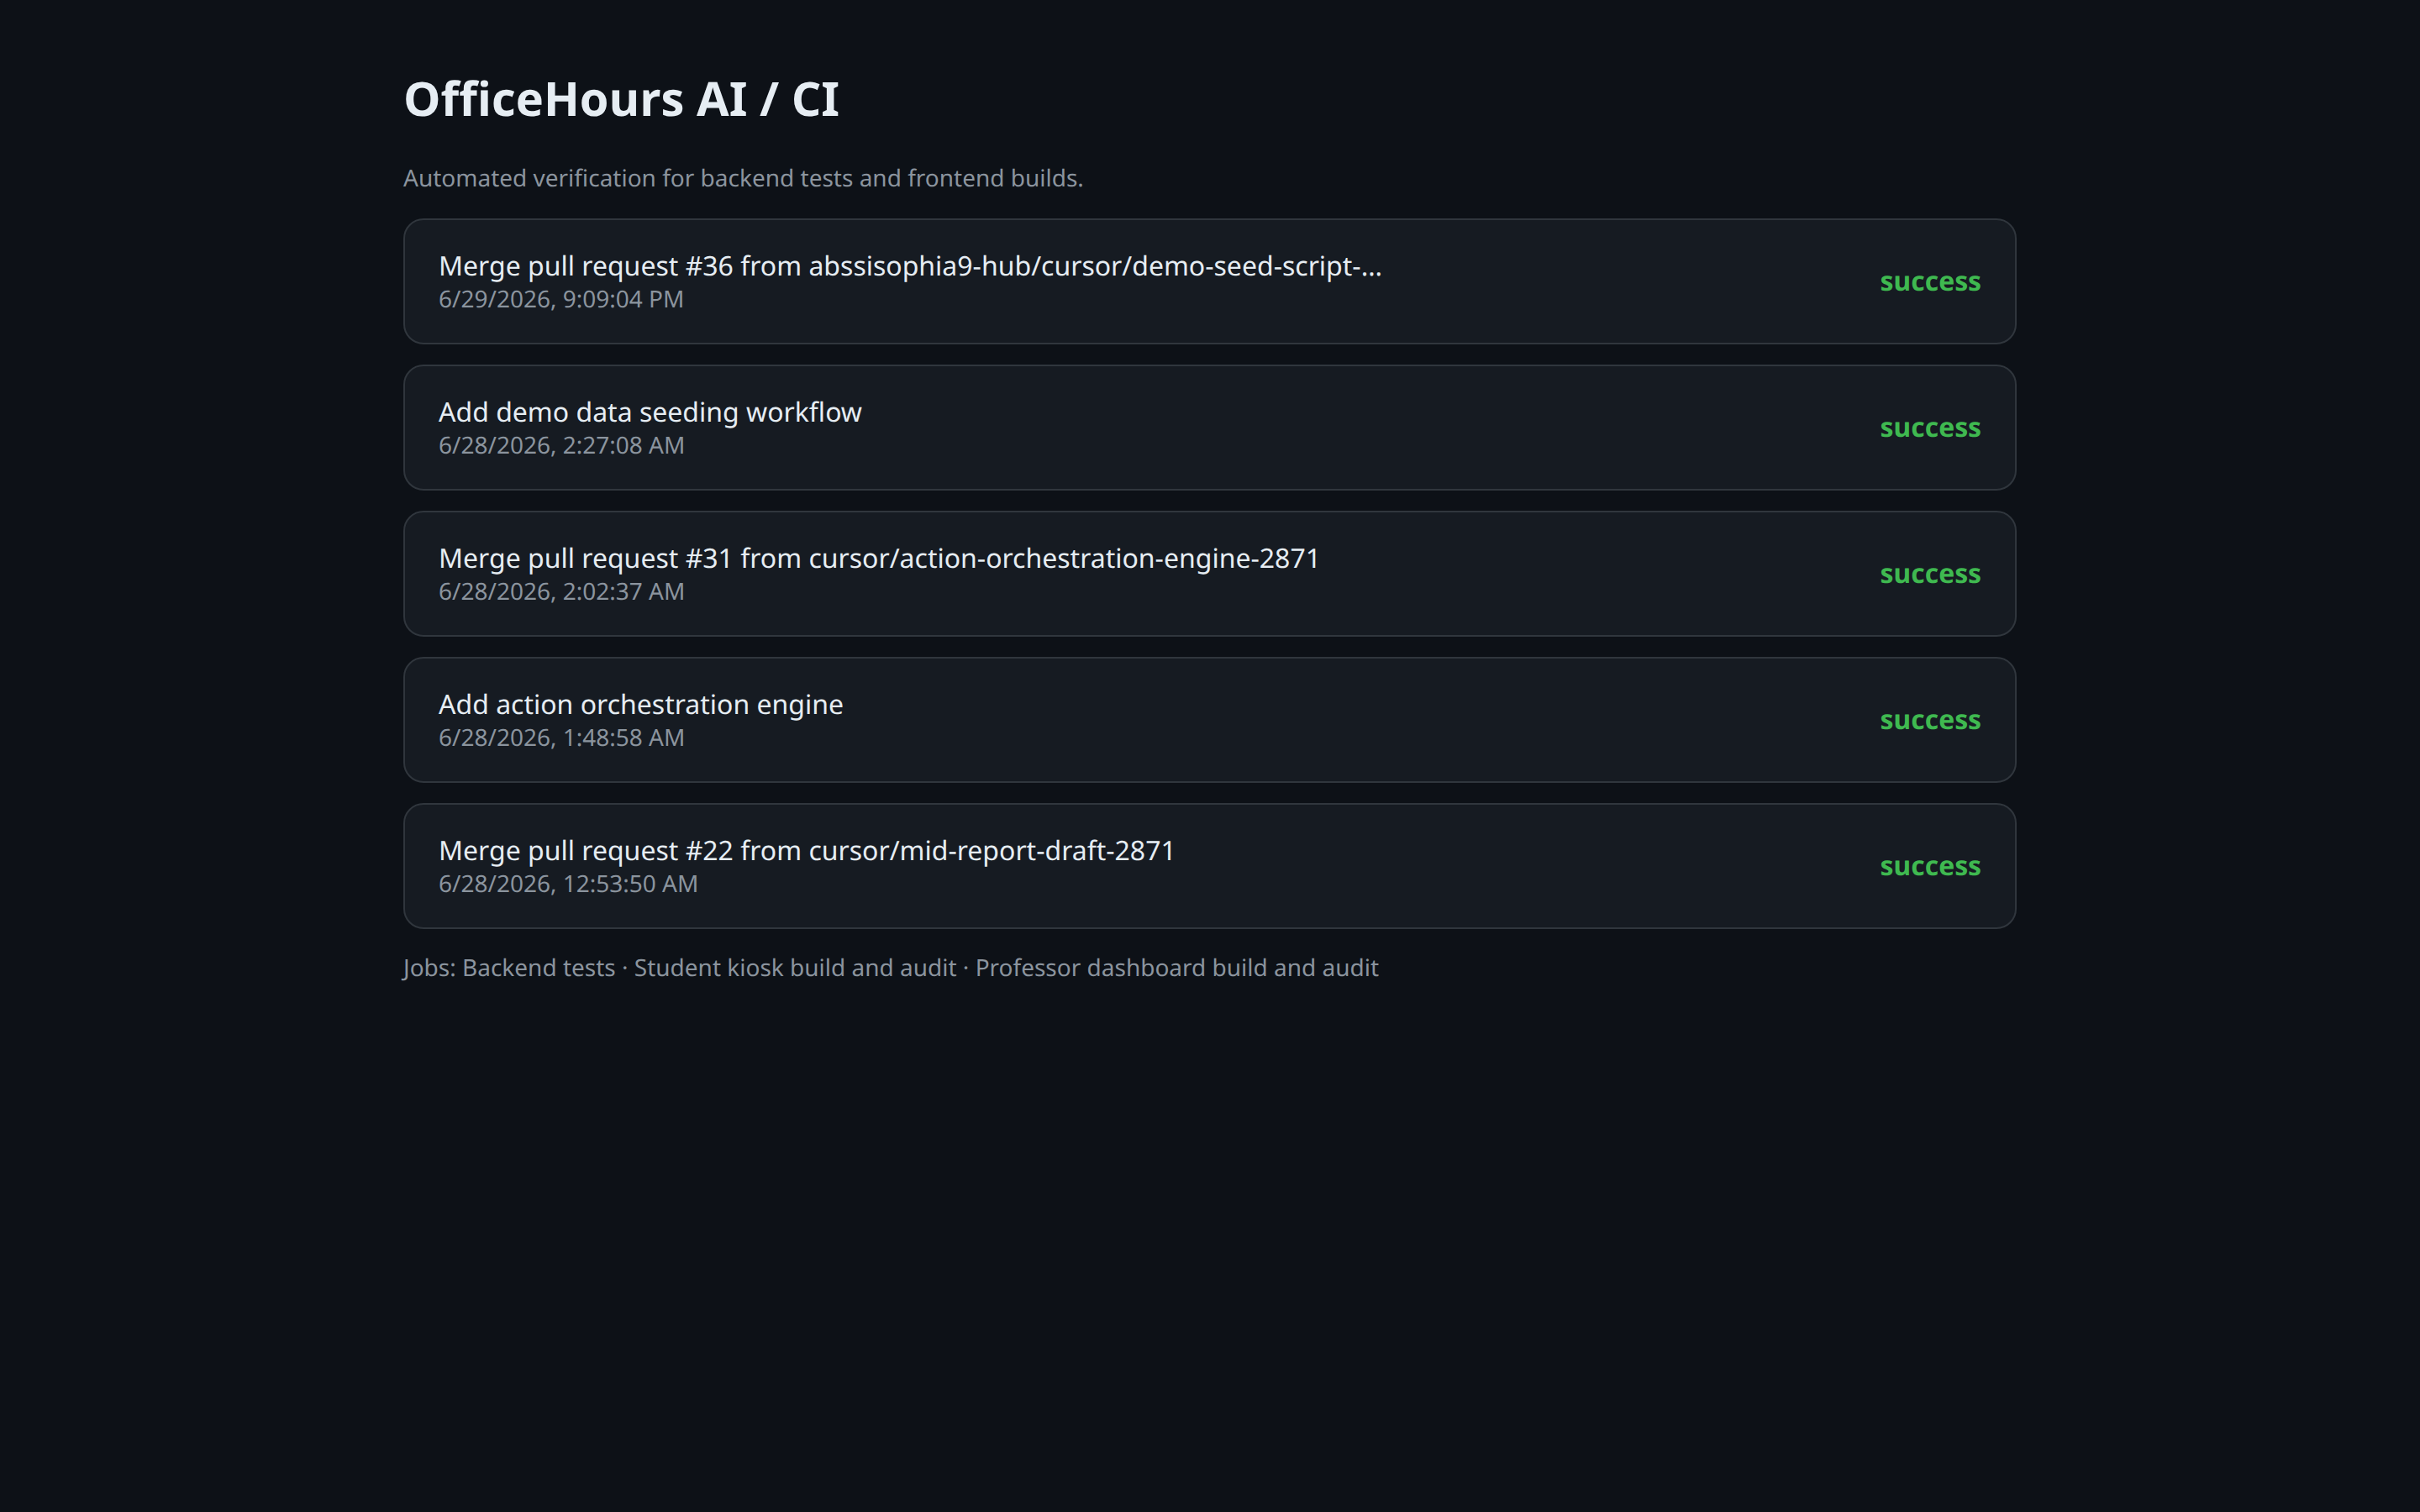
\includegraphics[width=0.92\linewidth]{../../demo/screenshots/08-github-actions-ci.png}
  \caption{Automated verification for backend and frontend builds.}
  \label{fig:ci}
\end{figure}

\section{Ethics and privacy}
The kiosk defaults to anonymous submission, stores student IDs only when opted
in, and keeps professor approval in the workflow. Development uses synthetic
data only.

\section{Evaluation plan}
Technical evaluation covers classifier accuracy, clustering behavior, CI, and
demo latency. User evaluation uses the student and professor post-demo surveys
in \path{docs/surveys/}.

\section{Remaining work at mid-semester checkpoint}
Near-term items included backend office-hours persistence, action-plan export,
anonymous status lookup, pilot survey collection, and final-report preparation.
Several of these were completed after this mid-report draft.

\section{Conclusion}
The prototype demonstrates the core workflow from student submission through
clustered professor recommendations. The screenshots above provide evidence of
a functional MVP suitable for simulated finals-week evaluation.

\end{document}
